\documentclass[12pt,twoside,a4paper]{article}
%\usepackage{lexend}

%\usepackage[131-134]{pagesel} 
%\usepackage[131-133]{pagesel} 

\usepackage{fancyhdr} %Paket laden
\usepackage{listings}
%\usepackage[UTF8]{inputenc}
\usepackage{multirow} 
\usepackage{color}
\usepackage{rotating}
\usepackage{hyperref}
\usepackage{amssymb}
\usepackage{amsmath}
\usepackage{hyperref}
\hypersetup{colorlinks,    linkcolor=black}
\usepackage{enumitem,amssymb}
\newlist{todolist}{itemize}{2}
\setlist[todolist]{label=$\square$}
\usepackage{menukeys}


\usepackage{makeidx}
\def\mmakeidx{1}
\makeindex 

\usepackage{minitoc}

%\usepackage[german]{babel}

% https://tex.stackexchange.com/questions/10255/xml-syntax-highlighting



\definecolor{gray}{rgb}{0.4,0.4,0.4}
\definecolor{darkblue}{rgb}{0.0,0.0,0.6}
\definecolor{cyan}{rgb}{0.0,0.6,0.6}

\lstset{
  basicstyle=\ttfamily,
  columns=fullflexible,
  showstringspaces=false,
  commentstyle=\color{gray}\upshape
}

\lstdefinelanguage{XML}
{
  morestring=[b]",
  morestring=[s]{>}{<},
  morecomment=[s]{<?}{?>},
  stringstyle=\color{black},
  identifierstyle=\color{darkblue},
  keywordstyle=\color{cyan},
numbers=left,
  numberstyle = \tiny,
  morekeywords={xmlns,version,type}% list your attributes here
}



\title{A  Five-Motor Robotic Platform \linebreak for Software Training Application}
\author{Christoph Kendel}


\begin{document}


    \maketitle
    \begin{abstract}
Students often express dissatisfaction with robot car kits and  simulated environments, arguing that these do not represent ``real" robotics. However, identifying a hands-on project that offers at least five degrees of freedom, millimeter-level precision, and minimal risk of damage has proven challenging.

The  {\bf 5Motor}  robot addresses this gap by providing a cost-effective, accessible platform that supports programming via G-code, either directly or through a Python wrapper. Its open architecture enables students to engage with a wide range of robotics concepts  --- including kinematics, motion control, and video analysis  --- making it a practical and educational tool for robotics training.
    \end{abstract}

\pagebreak



\section{Hardware}

The 3D printed needs for accuracy metal components for all contact joints.  So ball bearings and  linear bearings (MGN09) are used. Only one type of motor is used
for all axis: a Nema14 pancake stepper motor.



\begin{figure}[h!]
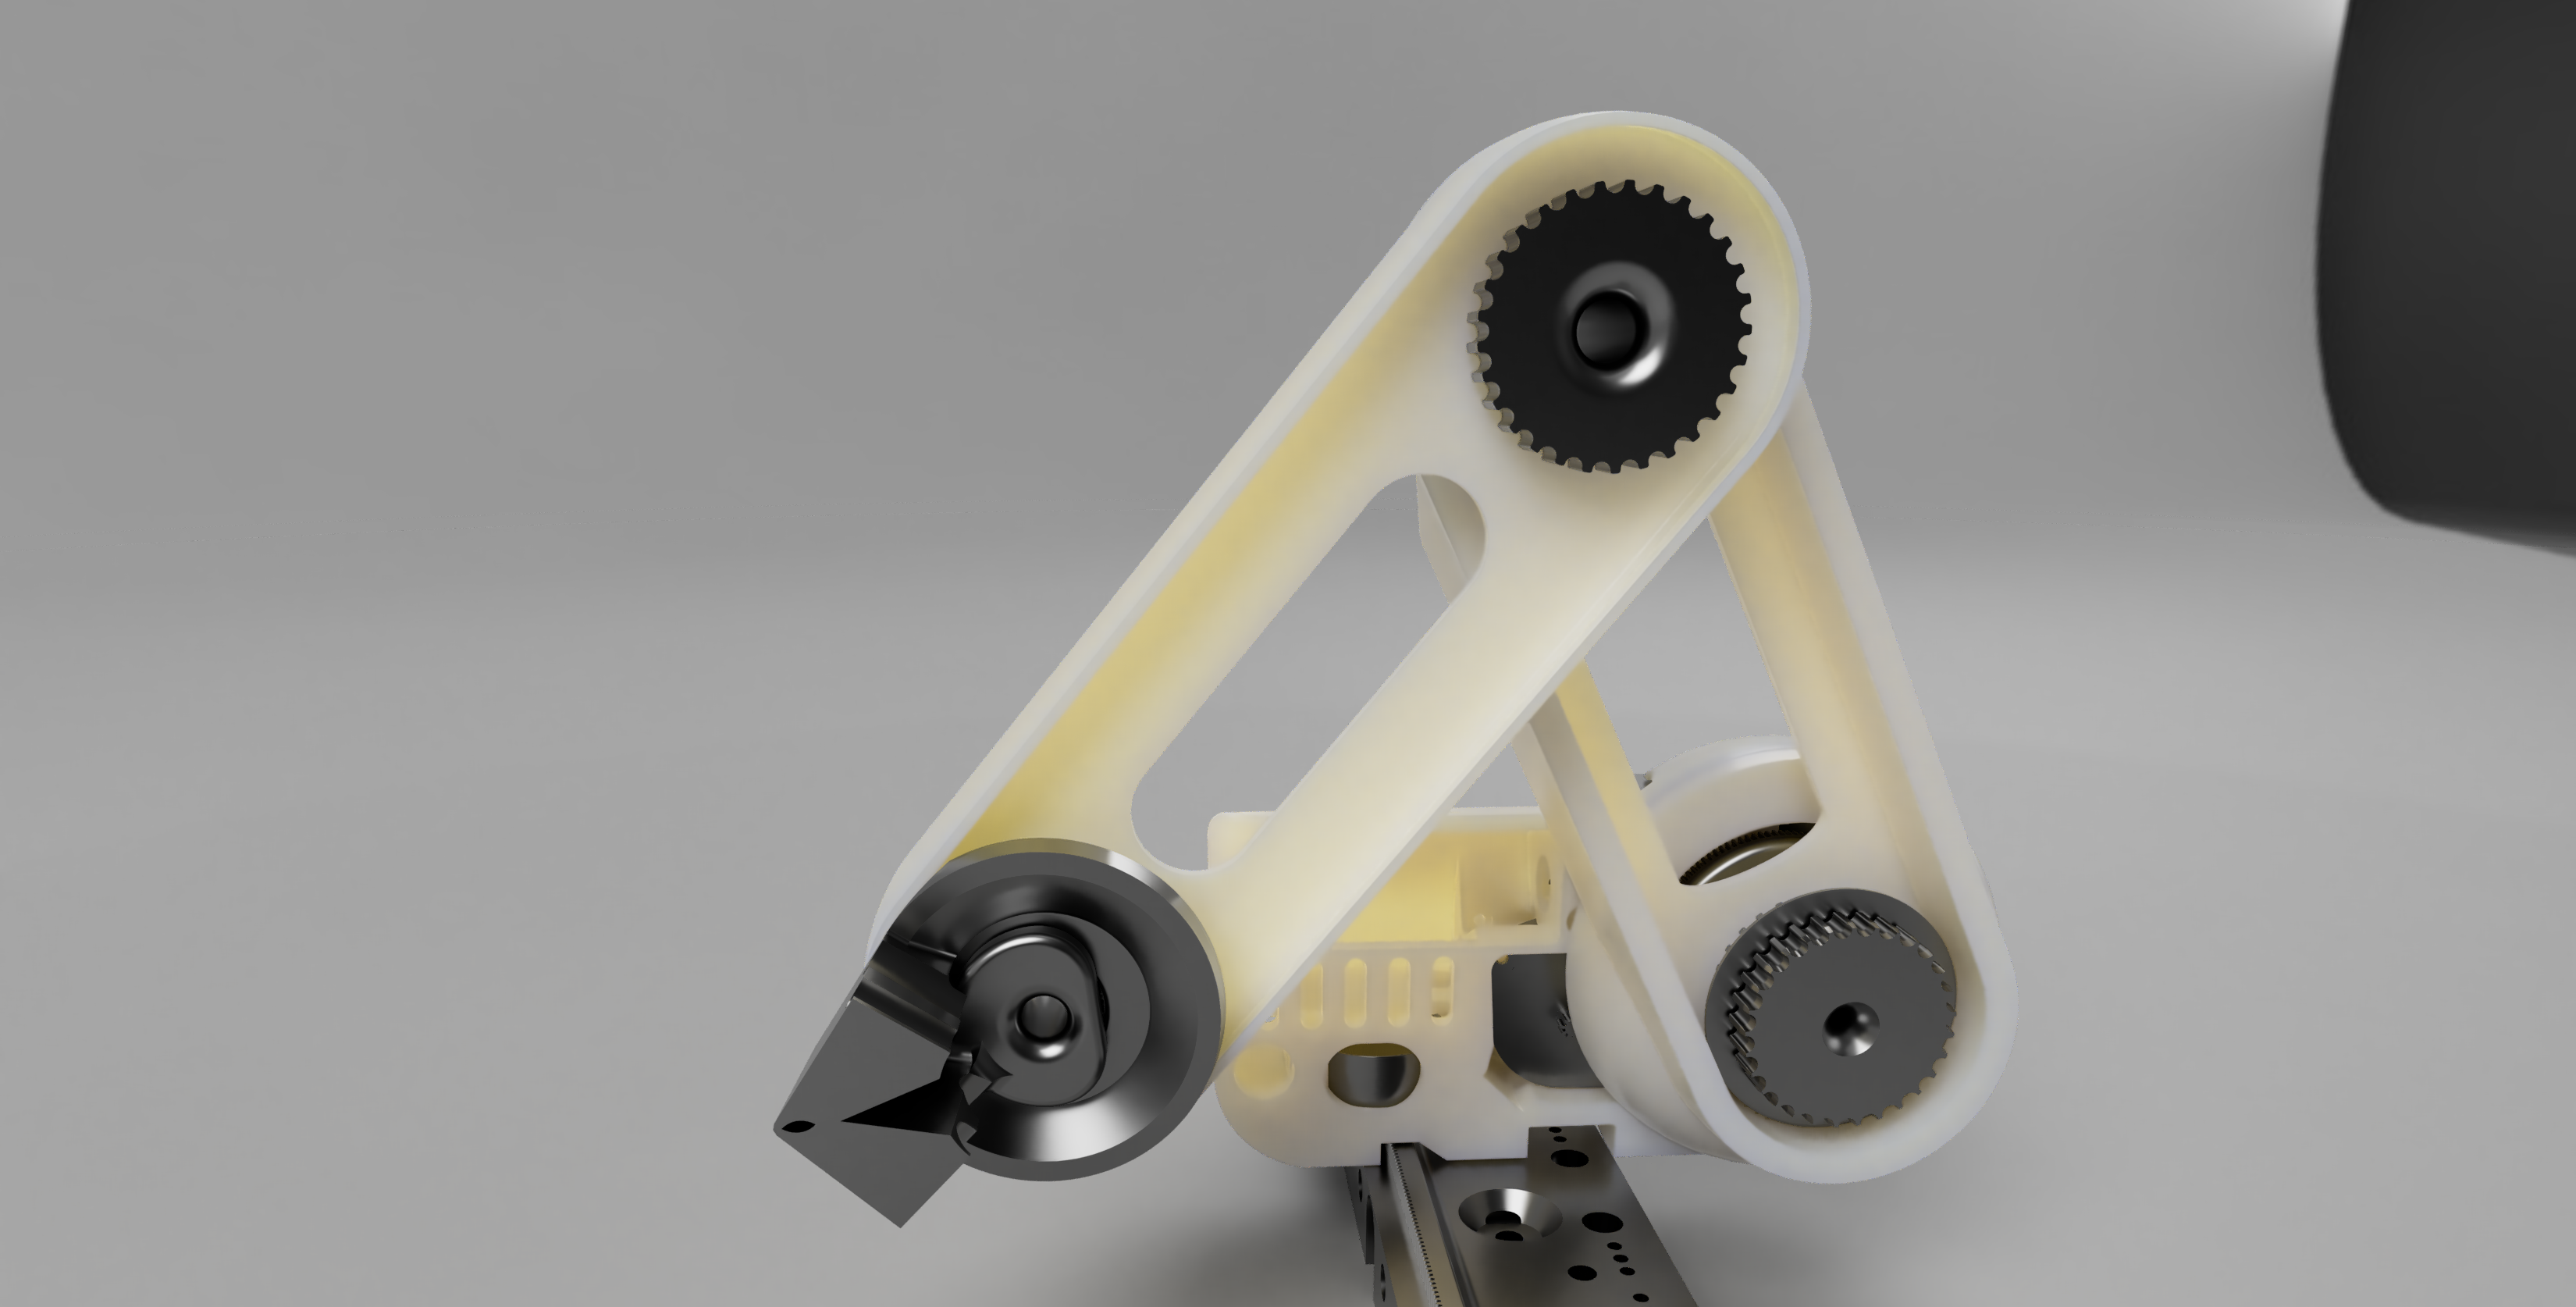
\includegraphics[width=\linewidth]{Pictures/01_SideView_a.png}
\caption{Rendering of the 5Motor robot}
\end{figure}

The design  allows students to do mistakes. If a hard limit is ignored, the force of the motors is small so it just  crashes into the wall  with just loosing allignment, and not causing damage.  This minimal  force has as a consequence, that the motors for the hand motion can not be lifted in the upper arm%
%
\footnote{any motor in the upper or lower arm would demand a stronger  motor in the shoulder, and thus the danger of damage.}.
% 
 Thus the movement is transmitted via 
HTD 5M belts, so the belt drivers can be printed.

The Robot can be seen in action on   \href{https://youtu.be/BwlxCkYBifw}{youtu.be/BwlxCkYBifw}. The 3D files are published on  \href{https://github.com/ChKendel/5Motor}{github.com/ChKendel/5Motor}.



 \section{Firmware}

The  Robot is running \href{https://github.com/bdring/FluidNC}{FluidNC} to receive GCode and send current to the motors. The board is based on an  ESP32 
and some TMC2209 Drivers. 

\section{Python Software} 

Students can either use the GCode directly on the firmware. Or use a python wrapper for more sophisticated kinematics.


\end{document}